\section{\RU{Если вариантов мало}\EN{Small number of cases}}

\lstinputlisting{patterns/08_switch/1_few/few.c}

\EN{\subsubsection{x86}

\myparagraph{\NonOptimizing MSVC}

Result (MSVC 2010):

\lstinputlisting[caption=MSVC 2010]{patterns/08_switch/1_few/few_msvc.asm}

Our function with a few cases in switch() is in fact analogous to this construction:

\lstinputlisting[label=switch_few_ifelse]{patterns/08_switch/1_few/few_analogue.c}

\myindex{\CLanguageElements!switch}
\myindex{\CLanguageElements!if}

If we work with switch() with a few cases it is impossible to be sure if it was
a real switch() in the source code, or just a pack of if() statements.
\myindex{\SyntacticSugar}

This implies that switch() is like syntactic sugar for a large number of nested if()s.

There is nothing especially new to us in the generated code,
with the exception of the compiler moving input variable $a$ to a temporary local variable \TT{tv64}
\footnote{Local variables in stack are prefixed with \TT{tv}---that's how MSVC names internal variables for its needs}.

If we compile this in GCC 4.4.1, we'll get almost the same result, even with maximal optimization
turned on (\Othree option).

\myparagraph{\Optimizing MSVC}

% TODO separate various kinds of \TT
% idea: enclose command lines in a specific environment, like \cmdline{} 
% assembly instructions in \asm{} (now both \TT and \q{} are used),
% variables in,  like \var{}
% messages (string constants) in something else, like \strconst
% to separate them all. Now they all use \TT, which is not best
% \INS{} for all instructions including operands? --DY
Now let's turn on optimization in MSVC (\Ox): \TT{cl 1.c /Fa1.asm /Ox}

\label{JMP_instead_of_RET}
\lstinputlisting[caption=MSVC]{patterns/08_switch/1_few/few_msvc_Ox.asm}

Here we can see some dirty hacks.

\myindex{x86!\Instructions!JZ}
\myindex{x86!\Instructions!JE}
\myindex{x86!\Instructions!SUB}

First: the value of $a$ is placed in \EAX and 0 is subtracted from it. Sounds absurd, but it is done to check if 
the value in \EAX was 0. If yes, the \ZF flag is to be set (e.g. subtracting from 0 is 0) 
and the first conditional jump \JE (\IT{Jump if Equal} or synonym \JZ~---\IT{Jump if Zero}) is to be triggered 
and control flow is to be passed to the \TT{\$LN4@f} label, where the \TT{'zero'} message is being printed. 
If the first jump doesn't get triggered, 1 is subtracted from the input value and if at some stage the result is 0, 
the corresponding jump is to be triggered.

And if no jump gets triggered at all, the control flow passes to \printf with string argument \\
\TT{'something unknown'}.

\label{jump_to_last_printf}
\myindex{\Stack}

Second: we see something unusual for us: a string pointer is placed into the $a$ variable, and 
then \printf is called not via \CALL, but via \JMP. There is a simple explanation for that: 
the \gls{caller} pushes a value to the stack and calls our function via \CALL. 
\CALL itself pushes the return address (\ac{RA}) to the stack and does an unconditional jump to our function address. 
Our function at any point of execution (since it do not contain any instruction that moves the stack 
pointer) has the following stack layout:

\begin{itemize}
\item\ESP---points to \ac{RA}
\item\TT{ESP+4}---points to the $a$ variable 
\end{itemize}

On the other side, when we need to call \printf here we need exactly the same stack 
layout, except for the first \printf argument, which needs to point to the string. 
And that is what our code does.

It replaces the function's first argument with the address of the string and 
jumps to \printf, as if we didn't call our function \ttf, but directly \printf.
\printf prints a string to \gls{stdout} and then executes the \RET instruction, which POPs 
\ac{RA} from the stack and control flow is returned not to \ttf but rather to \ttf's \gls{callee}, 
bypassing the end of the \ttf function.

\myindex{\CStandardLibrary!longjmp()}
\newcommand{\URLSJ}{\href{http://go.yurichev.com/17121}{wikipedia}}

All this is possible because \printf is called right at the end of the \ttf function in all cases. 
In some way, it is similar to the \TT{longjmp()}\footnote{\URLSJ} function.
And of course, it is all done for the sake of speed.

A similar case with the ARM compiler is described in \q{\PrintfSeveralArgumentsSectionName}
section, here~(\myref{ARM_B_to_printf}).

\clearpage
\myparagraph{\olly}

Since this example is tricky, let's trace it in \olly.

\olly can detect such switch() constructs, and it can add some useful comments.
\EAX is 2 in the beginning, that's the function's input value: 

\begin{figure}[H]
\centering
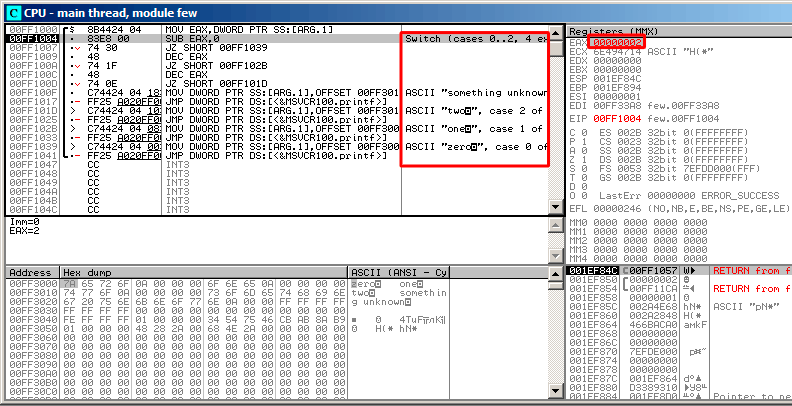
\includegraphics[scale=\FigScale]{patterns/08_switch/1_few/olly1.png}
\caption{\olly: \EAX 
now contain the first (and only) function argument}
\label{fig:switch_few_olly1}
\end{figure}

\clearpage
0 is subtracted from 2 in \EAX. 
Of course, \EAX still contains 2.
But the \ZF flag is now 0, indicating that the resulting value is non-zero:

\begin{figure}[H]
\centering
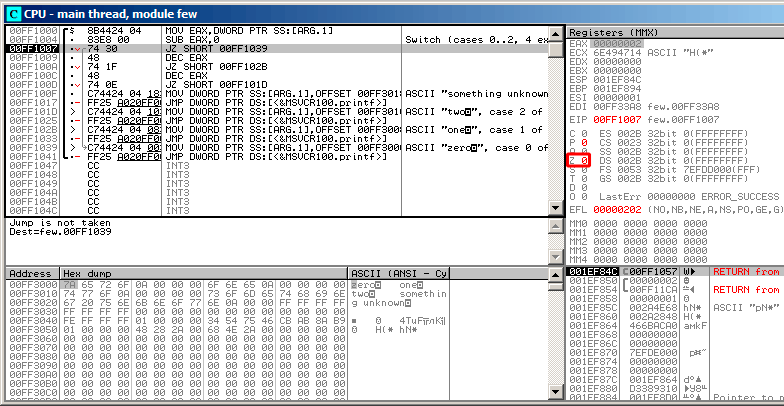
\includegraphics[scale=\FigScale]{patterns/08_switch/1_few/olly2.png}
\caption{\olly: \SUB executed}
\label{fig:switch_few_olly2}
\end{figure}

\clearpage
\DEC is executed and \EAX now contains 1. 
But 1 is non-zero, so the \ZF flag is still 0:

\begin{figure}[H]
\centering
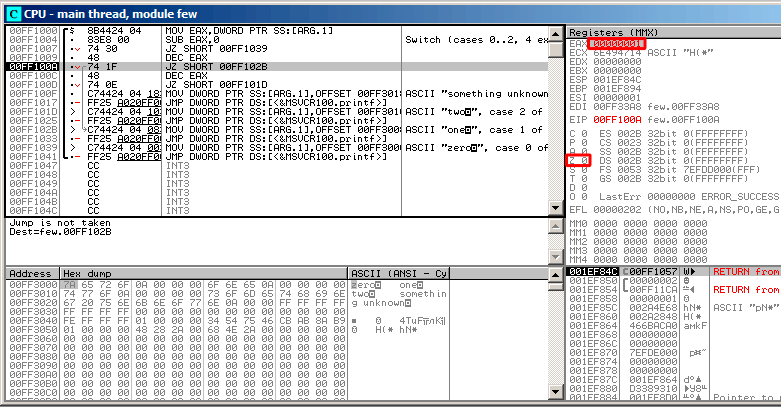
\includegraphics[scale=\FigScale]{patterns/08_switch/1_few/olly3.png}
\caption{\olly: first \DEC executed}
\label{fig:switch_few_olly3}
\end{figure}

\clearpage
Next \DEC is executed. 
\EAX is finally 0 and the \ZF flag gets set, because the result is zero:

\begin{figure}[H]
\centering
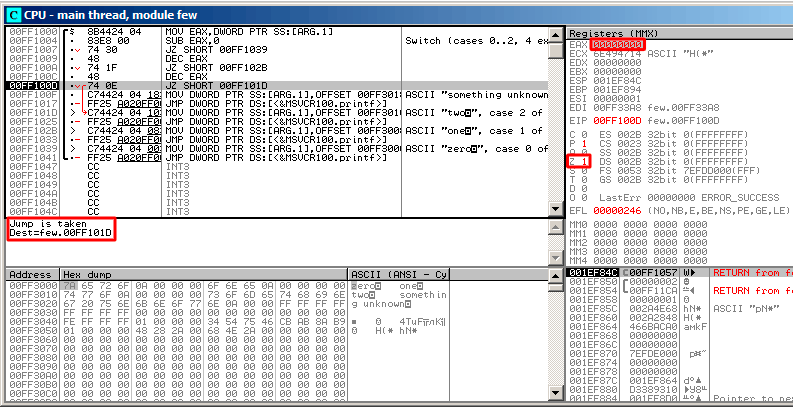
\includegraphics[scale=\FigScale]{patterns/08_switch/1_few/olly4.png}
\caption{\olly: second \DEC executed}
\label{fig:switch_few_olly4}
\end{figure}

\olly shows that this jump is to be taken now.

\clearpage
A pointer to the string \q{two} is to be written into the stack now:

\begin{figure}[H]
\centering
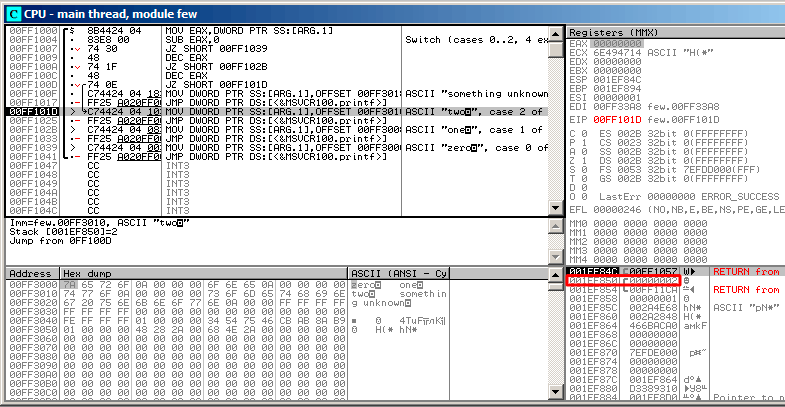
\includegraphics[scale=\FigScale]{patterns/08_switch/1_few/olly5.png}
\caption{\olly: 
pointer to the string is to be written at the place of the first argument}
\label{fig:switch_few_olly5}
\end{figure}

% TODO: homogenize numbers
% now they are inconsistent: sometimes plain text, sometimes in math mode
% some kind of \expr{} both for numbers and expressions? --DY
Please note: the current argument of the function is 2 and 2 is now in the stack at the address \TT{0x001EF850}.

\clearpage
\MOV writes the pointer to the string at address \TT{0x001EF850} (see the stack window).
Then, jump happens.
This is the first instruction of the \printf function in MSVCR100.DLL (This example was compiled with /MD switch): 

\begin{figure}[H]
\centering
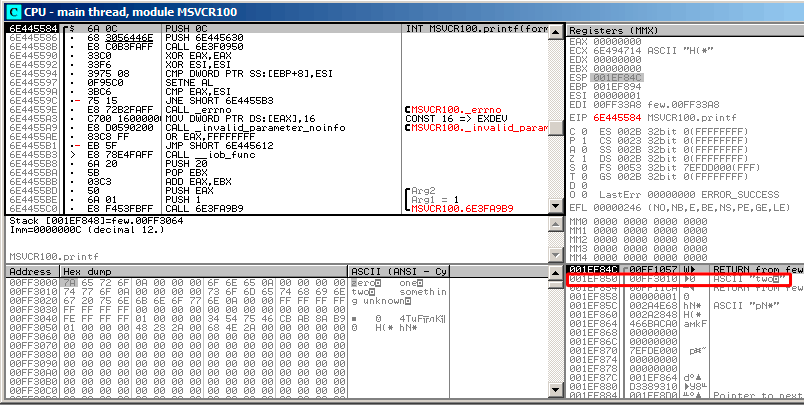
\includegraphics[scale=\FigScale]{patterns/08_switch/1_few/olly6.png}
\caption{\olly: first instruction of \printf \InENRU MSVCR100.DLL}
\label{fig:switch_few_olly6}
\end{figure}

Now \printf treats the string at \TT{0x00FF3010} as its only argument and prints the string.

\clearpage
This is the last instruction of \printf:

\begin{figure}[H]
\centering
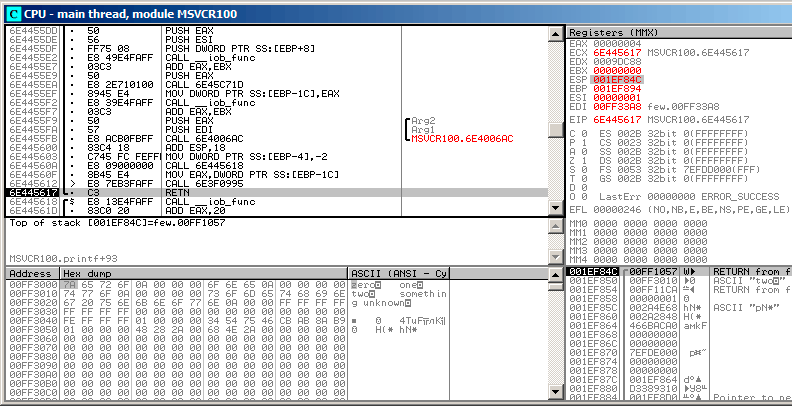
\includegraphics[scale=\FigScale]{patterns/08_switch/1_few/olly7.png}
\caption{\olly: last instruction of \printf in MSVCR100.DLL}
\label{fig:switch_few_olly7}
\end{figure}

The string \q{two} was just printed to the console window.

\clearpage
Now let's press F7 or F8 (\stepover) and return\dots not to \ttf , but rather to \main:

\begin{figure}[H]
\centering
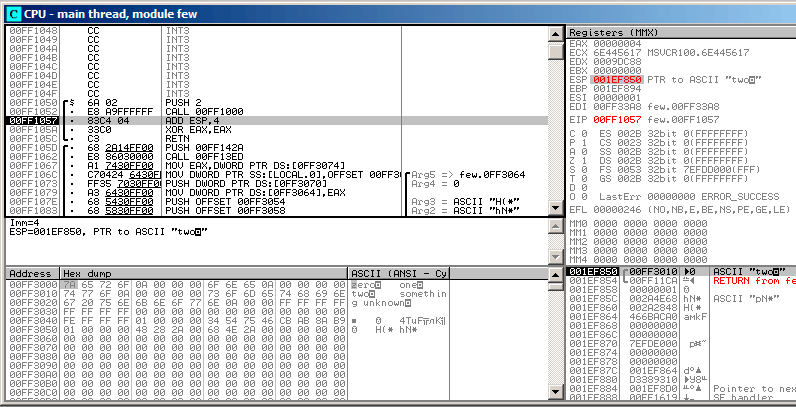
\includegraphics[scale=\FigScale]{patterns/08_switch/1_few/olly8.png}
\caption{\olly: return to \main}
\label{fig:switch_few_olly8}
\end{figure}

Yes, the jump was direct, from the guts of \printf to \main.
Because \ac{RA} in the stack points not to some place in \ttf , but rather to \main.
And \CALL \TT{0x00FF1000} was the actual instruction which called \ttf.



}
\RU{\subsubsection{x86}

\myparagraph{\NonOptimizing MSVC}

Это дает в итоге (MSVC 2010):

\lstinputlisting[caption=MSVC 2010]{patterns/08_switch/1_few/few_msvc.asm}

Наша функция со оператором switch(), с небольшим количеством вариантов, 
это практически аналог подобной конструкции:

\lstinputlisting[label=switch_few_ifelse]{patterns/08_switch/1_few/few_analogue.c}

\myindex{\CLanguageElements!switch}
\myindex{\CLanguageElements!if}
Когда вариантов немного и мы видим подобный код, невозможно сказать с уверенностью, был ли
в оригинальном исходном коде switch(), либо просто набор операторов if().

\myindex{\SyntacticSugar}
То есть, switch() это синтаксический сахар для большого количества вложенных проверок 
при помощи if().

В самом выходном коде ничего особо нового, 
за исключением того, что компилятор зачем-то 
перекладывает входящую переменную ($a$) во временную в локальном стеке \TT{v64}\footnote{Локальные переменные в стеке с префиксом \TT{tv}~--- 
так MSVC называет внутренние переменные для своих нужд}.

Если скомпилировать это при помощи GCC 4.4.1, то будет почти то же самое, даже с максимальной оптимизацией (ключ \Othree).

\myparagraph{\Optimizing MSVC}

% TODO separate various kinds of \TT
% idea: enclose command lines in a specific environment, like \cmdline{} 
% assembly instructions in \asm{} (now both \TT and \q{} are used),
% variables in,  like \var{}
% messages (string constants) in something else, like \strconst
% to separate them all. Now they all use \TT, which is not best
% \INS{} for all instructions including operands? --DY

Попробуем включить оптимизацию кодегенератора MSVC (\Ox): \TT{cl 1.c /Fa1.asm /Ox}

\label{JMP_instead_of_RET}
\lstinputlisting[caption=MSVC]{patterns/08_switch/1_few/few_msvc_Ox.asm}

Вот здесь уже всё немного по-другому, причем не без грязных трюков.

\myindex{x86!\Instructions!JZ}
\myindex{x86!\Instructions!JE}
\myindex{x86!\Instructions!SUB}
Первое: \TT{а} помещается в \EAX и от него отнимается 0. Звучит абсурдно, но нужно это для того, чтобы проверить, 
0 ли в \EAX был до этого? Если да, то выставится флаг \ZF (что означает, что результат вычитания 0 от числа 
стал 0) и первый условный переход \JE (\IT{Jump if Equal} или его синоним \JZ~--- \IT{Jump if Zero}) 
сработает на метку \TT{\$LN4@f}, где выводится сообщение \TT{'zero'}.
Если первый переход не сработал, от значения отнимается по единице, 
и если на какой-то стадии в результате образуется 0, то сработает соответствующий переход.

И в конце концов, если ни один из условных переходов не сработал, управление передается \printf
со строковым аргументом \TT{'something unknown'}.

\label{jump_to_last_printf}
\myindex{\Stack}
Второе: мы видим две, мягко говоря, необычные вещи: указатель на сообщение помещается в переменную $a$, 
и затем \printf вызывается не через \CALL, а через \JMP. Объяснение этому простое. 
Вызывающая функция заталкивает в стек некоторое значение и через \CALL вызывает нашу функцию. 
\CALL в свою очередь заталкивает в стек адрес возврата (\ac{RA}) и делает безусловный переход на адрес нашей функции. 
Наша функция в самом начале (да и в любом её месте, потому что в теле функции нет ни одной инструкции, 
которая меняет что-то в стеке или в \ESP) имеет следующую разметку стека:

\begin{itemize}
\item\ESP --- хранится \ac{RA}
\item\TT{ESP+4} --- хранится значение $a$ 
\end{itemize}

С другой стороны, чтобы вызвать \printf, нам нужна почти такая же разметка стека, 
только в первом аргументе нужен указатель на строку. Что, собственно, этот код и делает.

Он заменяет свой первый аргумент на адрес строки, и затем передает управление \printf, как если бы вызвали не 
нашу функцию \ttf, а сразу \printf. 
\printf выводит некую строку на \gls{stdout}, затем исполняет инструкцию \RET, 
которая из стека достает \ac{RA} и управление передается в ту функцию, 
которая вызывала \ttf, минуя при этом конец функции \ttf.

\myindex{\CStandardLibrary!longjmp()}
\newcommand{\URLSJ}{\href{http://go.yurichev.com/17121}{wikipedia}}
Всё это возможно, потому что \printf вызывается в \ttf в самом конце. 
Всё это чем-то даже похоже на \TT{longjmp()}\footnote{\URLSJ}.
И всё это, разумеется, сделано для экономии времени исполнения.

Похожая ситуация с компилятором для ARM описана в секции \q{\PrintfSeveralArgumentsSectionName}~(\myref{ARM_B_to_printf}).

\clearpage
\myparagraphold{\olly}

Так как этот пример немного запутанный, попробуем оттрассировать его в \olly.

\olly может распознавать подобные switch()-конструкции, так что он добавляет полезные комментарии.
\EAX в начале равен 2, это входное значение функции: 

\begin{figure}[H]
\centering
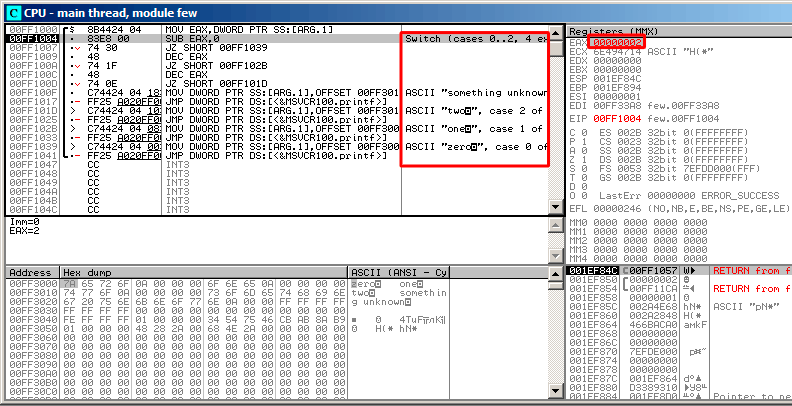
\includegraphics[scale=\FigScale]{patterns/08_switch/1_few/olly1.png}
\caption{\olly: \EAX содержит первый (и единственный) аргумент функции}
\label{fig:switch_few_olly1}
\end{figure}

\clearpage
0 отнимается от 2 в \EAX. 
Конечно же, \EAX всё ещё содержит 2.
Но флаг \ZF теперь 0, что означает, что последнее вычисленное значение не было нулевым:

\begin{figure}[H]
\centering
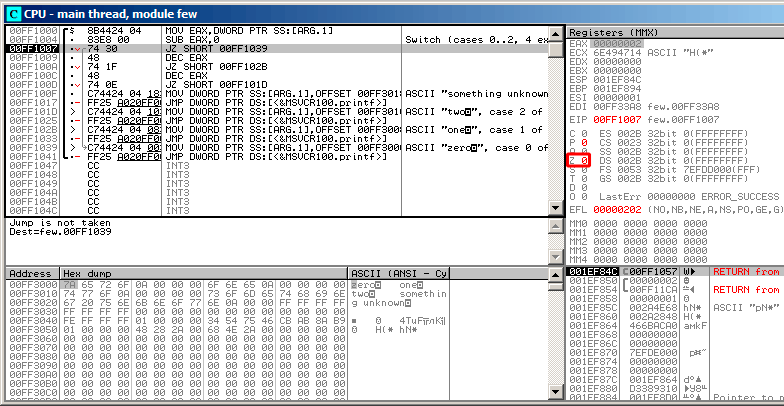
\includegraphics[scale=\FigScale]{patterns/08_switch/1_few/olly2.png}
\caption{\olly: \SUB исполнилась}
\label{fig:switch_few_olly2}
\end{figure}

\clearpage
\DEC исполнилась и \EAX теперь содержит 1. 
Но 1 не ноль, так что флаг \ZF всё ещё 0:

\begin{figure}[H]
\centering
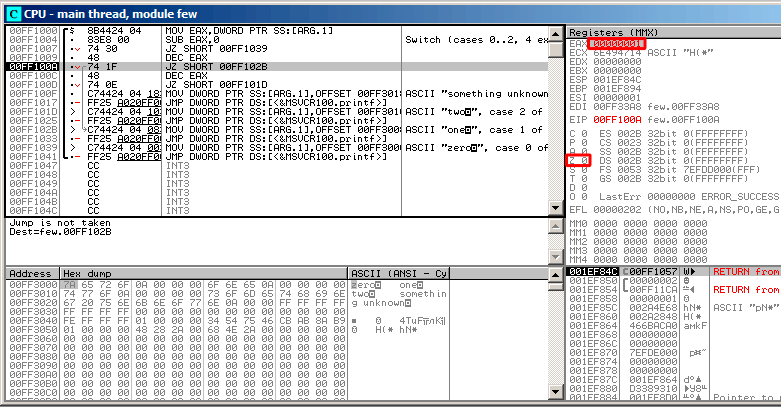
\includegraphics[scale=\FigScale]{patterns/08_switch/1_few/olly3.png}
\caption{\olly: первая \DEC исполнилась}
\label{fig:switch_few_olly3}
\end{figure}

\clearpage
Следующая \DEC исполнилась. 
\EAX наконец 0 и флаг \ZF выставлен, потому что результат~--- ноль:

\begin{figure}[H]
\centering
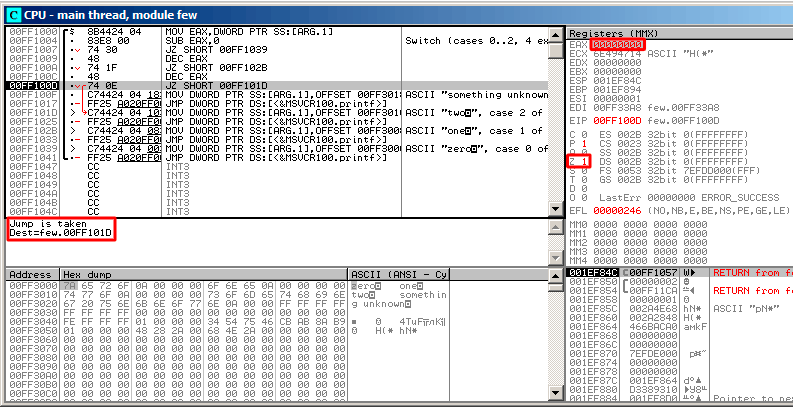
\includegraphics[scale=\FigScale]{patterns/08_switch/1_few/olly4.png}
\caption{\olly: вторая \DEC исполнилась}
\label{fig:switch_few_olly4}
\end{figure}

\olly показывает, что условный переход сейчас сработает.

\clearpage
Указатель на строку \q{two} 
сейчас будет записан в стек:

\begin{figure}[H]
\centering
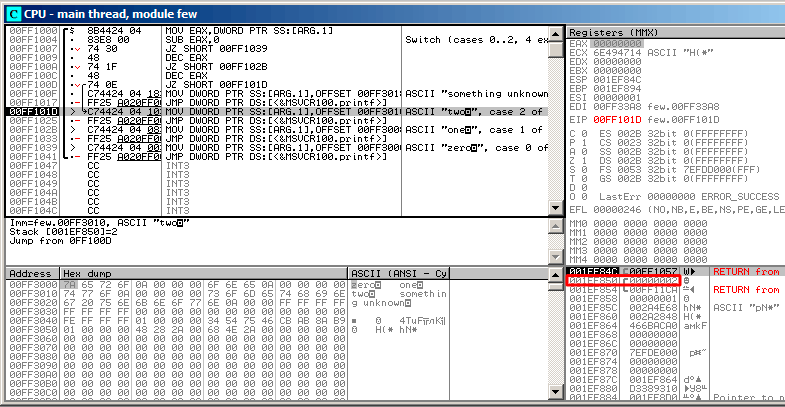
\includegraphics[scale=\FigScale]{patterns/08_switch/1_few/olly5.png}
\caption{\olly: указатель на строку сейчас запишется на место первого аргумента}
\label{fig:switch_few_olly5}
\end{figure}

% TODO: homogenize numbers
% now they are inconsistent: sometimes plain text, sometimes in math mode
% some kind of \expr{} both for numbers and expressions? --DY
Обратите внимание: текущий аргумент функции это 2 и 2 прямо сейчас в стеке по адресу \TT{0x001EF850}.

\clearpage
\MOV записывает указатель на строку по адресу \TT{0x001EF850} (см. окно стека).
Переход сработал.
Это самая первая инструкция функции \printf в MSVCR100.DLL (этот пример был скомпилирован с опцией /MD): 

\begin{figure}[H]
\centering
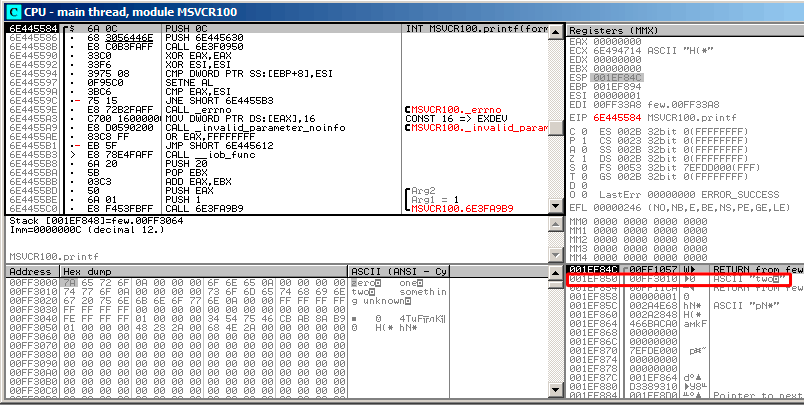
\includegraphics[scale=\FigScale]{patterns/08_switch/1_few/olly6.png}
\caption{\olly: первая инструкция в \printf в MSVCR100.DLL}
\label{fig:switch_few_olly6}
\end{figure}

Теперь \printf считает строку на \TT{0x00FF3010} как свой единственный аргумент и выводит строку.

\clearpage
Это самая последняя инструкция функции \printf:

\begin{figure}[H]
\centering
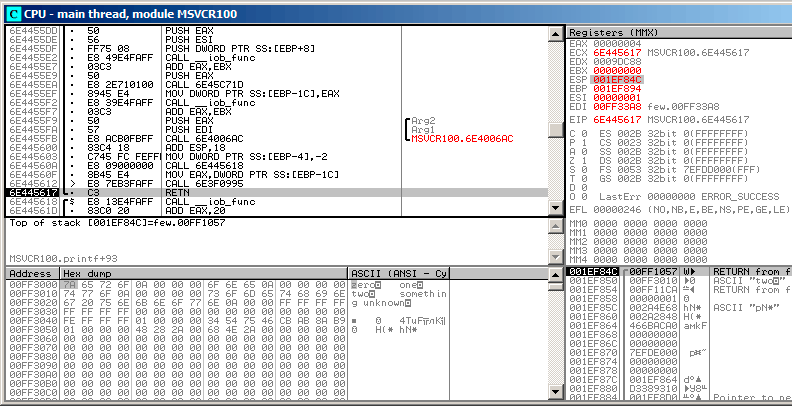
\includegraphics[scale=\FigScale]{patterns/08_switch/1_few/olly7.png}
\caption{\olly: последняя инструкция в \printf в MSVCR100.DLL}
\label{fig:switch_few_olly7}
\end{figure}

Строка \q{two} была только что выведена в консоли.

\clearpage
Нажмем F7 или F8 (\stepover) и вернемся\dots нет, не в функцию \ttf но в \main:

\begin{figure}[H]
\centering
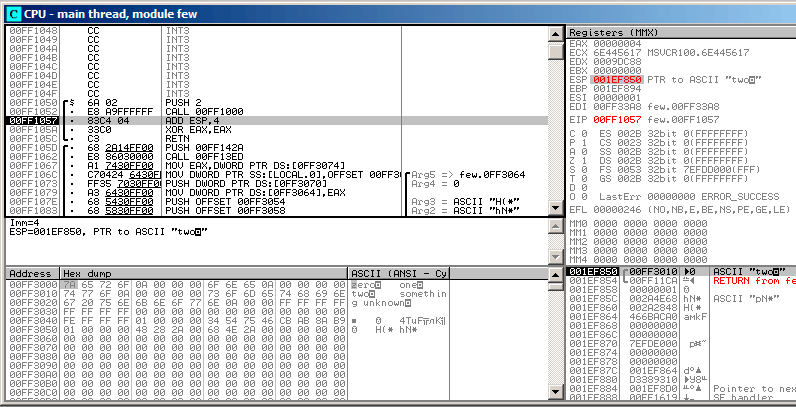
\includegraphics[scale=\FigScale]{patterns/08_switch/1_few/olly8.png}
\caption{\olly: возврат в \main}
\label{fig:switch_few_olly8}
\end{figure}

Да, это прямой переход из внутренностей \printf в \main.
Потому как \ac{RA} в стеке указывает не на какое-то место в функции \ttf а в \main.
И \CALL \TT{0x00FF1000} это инструкция вызывающая функцию \ttf.



}
\EN{\subsubsection{ARM: \OptimizingKeilVI (\ARMMode)}
\myindex{\CLanguageElements!switch}

\lstinputlisting{patterns/08_switch/1_few/few_ARM_ARM_O3.asm}

Again, by investigating this code we cannot say if it was a switch() in the original source code, 
or just a pack of if() statements.

\myindex{ARM!\Instructions!ADRcc}

Anyway, we see here predicated instructions again (like \ADREQ (\IT{Equal}))
which is triggered only in case $R0=0$, and then loads the address of the string \IT{<<zero\textbackslash{}n>>}
into \Reg{0}.
\myindex{ARM!\Instructions!BEQ}
The next instruction \ac{BEQ} redirects control flow to \TT{loc\_170}, if $R0=0$.

An astute reader may ask, will \ac{BEQ} trigger correctly since \ADREQ it
has already filled the \Reg{0} register before with another value?

Yes, it will since \ac{BEQ} checks the flags set by the \CMP instruction, 
and \ADREQ does not modify any flags at all.

The rest of the instructions are already familiar to us. 
There is only one call to \printf , at the end, and we have already examined this trick here~(\myref{ARM_B_to_printf}).
At the end, there are three paths to \printf{}.

\myindex{ARM!\Instructions!ADRcc}
\myindex{ARM!\Instructions!CMP}
The last instruction, \TT{CMP R0, \#2}, is needed to check if $a=2$.

If it is not true, then \ADRNE loads a pointer to the string \IT{<<something unknown \textbackslash{}n>>}
into \Reg{0}, since $a$ has already been checked to be equal to 0 or 1,
and we can sure that the $a$ variable is not equal to these numbers at this point.
And if $R0=2$, 
a pointer to the string \IT{<<two\textbackslash{}n>>}
will be loaded by \ADREQ into \Reg{0}.

\subsubsection{ARM: \OptimizingKeilVI (\ThumbMode)}

\lstinputlisting{patterns/08_switch/1_few/few_ARM_thumb_O3.asm}

% FIXME а каким можно? к каким нельзя? \myref{} ->

As was already mentioned, it is not possible to add conditional predicates to most instructions in Thumb
mode, so the Thumb-code here is somewhat similar to the easily understandable x86 \ac{CISC}-style code.

\subsubsection{ARM64: \NonOptimizing GCC (Linaro) 4.9}

\lstinputlisting{patterns/08_switch/1_few/ARM64_GCC_O0_EN.lst}

The type of the input value is \Tint, hence register \RegW{0} is used to hold it instead of the whole
\RegX{0} register.

The string pointers are passed to \puts using an \INS{ADRP}/\INS{ADD} instructions pair just like it was demonstrated in the 
\q{\HelloWorldSectionName} example:~\myref{pointers_ADRP_and_ADD}.

\subsubsection{ARM64: \Optimizing GCC (Linaro) 4.9}

\lstinputlisting{patterns/08_switch/1_few/ARM64_GCC_O3_EN.lst}

Better optimized piece of code.
\TT{CBZ} (\IT{Compare and Branch on Zero}) instruction does jump if \RegW{0} is zero.
There is also a direct jump to \puts instead of calling it, like it was explained before:~\myref{JMP_instead_of_RET}.

}
\RU{\subsectionold{ARM: \OptimizingKeilVI (\ARMMode)}
\myindex{\CLanguageElements!switch}

\lstinputlisting{patterns/08_switch/1_few/few_ARM_ARM_O3.asm}

Мы снова не сможем сказать, глядя на этот код, был ли в оригинальном исходном коде switch() 
либо же несколько операторов if().

\myindex{ARM!\Instructions!ADRcc}
Так или иначе, мы снова видим здесь инструкции с предикатами, например, \ADREQ (\IT{(Equal)}), 
которая будет исполняться только
если $R0=0$, и тогда в \Reg{0} будет загружен адрес строки \IT{<<zero\textbackslash{}n>>}.

\myindex{ARM!\Instructions!BEQ}
Следующая инструкция \ac{BEQ} перенаправит исполнение на \TT{loc\_170}, если $R0=0$.

Кстати, наблюдательный читатель может спросить, сработает ли \ac{BEQ} нормально,
ведь \ADREQ перед ним уже заполнила регистр \Reg{0} чем-то другим?

Сработает, потому что \ac{BEQ} проверяет флаги, установленные инструкцией \CMP, 
а \ADREQ флаги никак не модифицирует.

Далее всё просто и знакомо. 
Вызов \printf один, и в самом конце, мы уже рассматривали подобный трюк~(\myref{ARM_B_to_printf}).
К вызову функции \printf{} в конце ведут три пути.

\myindex{ARM!\Instructions!ADRcc}
\myindex{ARM!\Instructions!CMP}
Последняя инструкция \TT{CMP R0, \#2} здесь нужна, чтобы узнать $a=2$ или нет.

Если это не так, то при помощи \ADRNE (\IT{Not Equal}) в \Reg{0} будет загружен указатель на 
строку \IT{<<something unknown \textbackslash{}n>>}, ведь $a$ уже было проверено на 0 и 1 до этого, 
и здесь $a$ точно не попадает под эти константы.

Ну а если $R0=2$, в \Reg{0} будет загружен указатель на строку \IT{<<two\textbackslash{}n>>} при помощи инструкции \ADREQ.

\subsectionold{ARM: \OptimizingKeilVI (\ThumbMode)}

\lstinputlisting{patterns/08_switch/1_few/few_ARM_thumb_O3.asm}

% FIXME а каким можно? к каким нельзя? \myref{} ->
Как уже было отмечено, в Thumb-режиме нет возможности добавлять условные предикаты к большинству инструкций,
так что Thumb-код вышел похожим на код x86 в стиле \ac{CISC}, вполне понятный.

\subsectionold{ARM64: \NonOptimizing GCC (Linaro) 4.9}

\lstinputlisting{patterns/08_switch/1_few/ARM64_GCC_O0_RU.lst}

Входное значение имеет тип \Tint, поэтому для него используется регистр \RegW{0},
а не целая часть регистра \RegX{0}.

Указатели на строки передаются в \puts при помощи пары инструкций ADRP/ADD, как было показано в примере
\q{\HelloWorldSectionName}:~\myref{pointers_ADRP_and_ADD}.

\subsectionold{ARM64: \Optimizing GCC (Linaro) 4.9}

\lstinputlisting{patterns/08_switch/1_few/ARM64_GCC_O3_RU.lst}

Фрагмент кода более оптимизированный.
Инструкция \TT{CBZ} (\IT{Compare and Branch on Zero}~--- сравнить и перейти если ноль) совершает переход если \RegW{0} ноль.
Здесь также прямой переход на \puts вместо вызова, как уже было описано:~\myref{JMP_instead_of_RET}.

}
\EN{\subsubsection{MIPS}

\lstinputlisting[caption=\Optimizing GCC 4.4.5 (IDA)]{patterns/08_switch/1_few/MIPS_O3_IDA_EN.lst}

\myindex{MIPS!\Instructions!JR}

The function always ends with calling \puts, so here we see a jump to \puts (\INS{JR}: \q{Jump Register}) instead of \q{jump and link}.
We talked about this earlier: \myref{JMP_instead_of_RET}.

\myindex{MIPS!Load delay slot}
We also often see \INS{NOP} instructions after \INS{LW} ones.
This is \q{load delay slot}: another \IT{delay slot} in MIPS.
\myindex{MIPS!\Instructions!LW}

An instruction next to \INS{LW} may execute at the moment while \INS{LW} loads value from memory. 

However, the next instruction must not use the result of \INS{LW}.

Modern MIPS CPUs have a feature to wait if the next instruction uses result of \INS{LW}, so this is somewhat outdated,
but GCC still adds NOPs for older MIPS CPUs.
In general, it can be ignored.
}
\RU{\subsubsection{MIPS}

\lstinputlisting[caption=\Optimizing GCC 4.4.5 (IDA)]{patterns/08_switch/1_few/MIPS_O3_IDA_RU.lst}

\myindex{MIPS!\Instructions!JR}

Функция всегда заканчивается вызовом \puts, так что здесь мы видим переход на \puts (\INS{JR}: \q{Jump Register})
вместо перехода с сохранением \ac{RA} (\q{jump and link}).

Мы говорили об этом ранее: \myref{JMP_instead_of_RET}.

\myindex{MIPS!Load delay slot}
Мы также часто видим NOP-инструкции после \INS{LW}.
Это \q{load delay slot}: ещё один \IT{delay slot} в MIPS.
\myindex{MIPS!\Instructions!LW}
Инструкция после \INS{LW} может исполняться в тот момент, когда \INS{LW} загружает значение из памяти.

Впрочем, следующая инструкция не должна использовать результат \INS{LW}.

Современные MIPS-процессоры ждут, если следующая инструкция использует результат \INS{LW}, так что всё это уже
устарело, но GCC всё еще добавляет NOP-ы для более старых процессоров.

Вообще, это можно игнорировать.

}

\subsection{\Conclusion{}}

\EN{A \IT{switch()} with few cases is indistinguishable from an \IT{if/else} construction, for example:}
\RU{Оператор \IT{switch()} с малым количеством вариантов трудно отличим от применения конструкции \IT{if/else}:}
\lstref{switch_few_ifelse}.

